\chapter{Hero Worship}

As members of the church, we sometimes get into what is known as hero
worship.\footnote{Noun: Excessive admiration for someone.} We tend to put prophets
and apostles on pedestals to the point they are seen as higher than anyone else. I
dare say, sometimes we put them even above that of Jesus Christ Himself. Which I'm
sure you can see the problem with that. No one is greater than the Risen Lord. We
should watch what we say about propehts and apostles of the Lord, it is Him who they
serve, not the other way around.

This hero worship was evident in the times of Joseph Smith, and have continued onward
throughout the world in these latter days. Being said of the prophet Joseph:

\begin{displayquote}
Joseph Smith, the Prophet and Seer of the Lord, has done more, save Jesus only, 
for the salvation of men in this world, than any other man that ever lived in
it.\footnote{D\&C 135:3}
\end{displayquote}

These days, people praise the current prophet for revelation he receives. We see the
outcome of such revelations and sometimes it becomes confusing. Recently, they
stopped calling a program Home Teaching and are calling it Ministering. Instead of
monthly reports, and visiting every month, it has changed to every three months.
Times have changed, where once you gave a lesson at a person's home, now you can get
by with a simple facebook message or text message to them instead.

People see these changes and are impressed by the Lord's servant by the obvious
revelation that has been received. I will not say one way or the other what I believe
is revelation vs. a corporate decision. I have my own thoughts on the matter and I
will leave it at that.

Another recent revelation was combining the Elders Quorum and the High Priests Group
into one single Elders Quorum. While this feels like just a simple restructure due to
low attendance numbers, it is called a revelation.

The members of the church priase the prophet for these actions and are amazed at how
wonderful it is to be living in a time of current revelation from the Lord.

All the while, children are being neglected and one on one youth interviews continue 
to happen within the church.

The church has said that it is not a business. It is not a corporation where people
climb the ladder as it were, yet that is exactly how it looks when seen from the
outside.\footnote{Inside the Quorum of the Twelve: Misconceptions about an Apostle's
Service, lds.org, 10 August 2018}

Here is the business listing for the LDS Church.

\begin{figure}[h!]
  \centering
  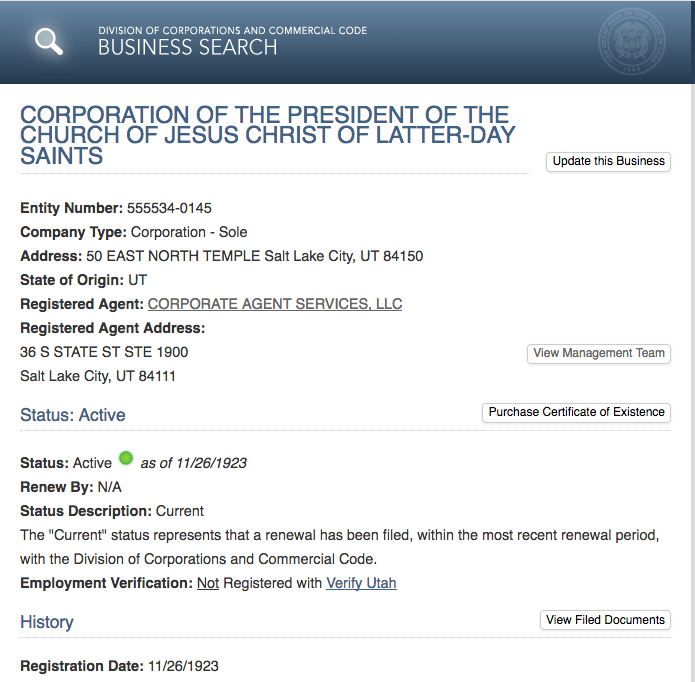
\includegraphics[width=1\linewidth]{articles/images/business.png}
  \caption{LDS Church Business Listing}
  \label{fig:business}
\end{figure}

Again, recently the church came out to declare that people shouldn't use the terms
``LDS" or ``Mormon" when speaking about the church. It should go by its full name.
``The Church of Jesus Christ of Latter-day Saints". Some people have gone to say that
by continuing to call yourself a Mormon, you are going against God's prophet and are
an apostate. With the constant use of the full church name, is that not saying
Christ's name too repeatedly?

According to scripture the Melchizedek Priesthood ``was called the Holy Priesthood, 
after the Order of the Son of God. But out of respect or reverence to the name of 
the Supreme Being, to avoid the too-frequent repetition of his name, 
they, the church, in the ancient days, called that priesthood after 
Melchizedek, or the Melchizedek Priesthood"\footnote{D\&C 107:3-4}

Is this not the same case? How can one be ``too-frequent repetition" and the other 
not?

Another interesting tidbit of information, The Church of Jesus Christ of Latter-day
Saints was known by the following names:

The Church of Christ (1830-1834)

The Church of the Latter Day Saints (1834)

The Church of Christ of Latter Day Saints (1836-1838)

The Lord finally in 1838 told Joseph what the correct name of the church would be:

\begin{displayquote}
For thus shall my church be called in the last days, even The Church of Jesus Chirst
of Latter-day Saints.\footnote{D\&C 115:4}
\end{displayquote}

Why did the Lord take so long in telling Joseph what the name of His church would be?
Is this not the same Lord who told Noah how to build an ark based on exact
dimensions? From 1820 to 1838, the Lord had not given Joseph the exact name of the
church by which it was to be called in these last days. I find that interesting.

The prophet's wife, Wendy Nelson said the following about the prophet:

\begin{displayquote}
``I have seen him changing in the last ten months," said Sister Nelson. ``It is as 
though he's been unleashed. He's free to finally do what he came to earth to do. ... 
And also, he's free to follow through with things he's been concerned about but 
could never do. Now that he's president of [the Church], he can do those
things."\footnote{Latter-day Saint Prophet, Wife and Apostle Share Insights 
of Global Ministry, Mormonnewsroom.org Article}
\end{displayquote}

From this quote, it would seem that President Nelson has had these thoughts and
changes in his mind for a while now, but now he can finally institute those changes.

An example of this was a talk he gave in 1990 General Conference.\footnote{April 1990 
Conference (Conference Report Page 17)} It had the same kinds of undertones about the 
name of the church. Six months later, President Hinckley noted the talk in another 
General Conference and then stated that the term Mormon was okay.\footnote{October 
1990 Conference (Conference Report Pages 68-69)}